\documentclass[12pt,a4paper]{extarticle}
\usepackage[margin=1.8cm,bottom=2cm]{geometry}
\usepackage{authblk}
\usepackage{float}
\usepackage{pdflscape}
\usepackage{graphicx}
\usepackage{booktabs}
\usepackage[hidelinks]{hyperref}
\usepackage[style=authoryear-icomp,
uniquelist=false,
maxnames=2,
minnames=1,
maxbibnames=99,
    backend=biber, giveninits=true,
    ibidtracker=false,
    uniquename=false,
    natbib=true]{biblatex}

\addbibresource{../battery_paper/DCE_lit_review.bib}
\addbibresource{../battery_paper/Used EV.bib}
\addbibresource{../battery_paper/EV battery.bib}
\addbibresource{../vehicle_paper/used_EV_lit_review.bib}

\AtEveryBibitem{%
  \clearfield{url}%
  \clearfield{urldate}%
  \clearfield{note}%
}

\setlength{\parskip}{2pt}

\renewcommand\Authfont{\fontsize{10}{12}\selectfont}
\renewcommand\Affilfont{\fontsize{10}{12}\selectfont}
\renewcommand\Authand{, }
\renewcommand\Authands{, }

\date{}

\begin{document}

\title{\fontsize{14}{17}\selectfont\textbf{Consumer Preferences in the Used Vehicle Market: Willingness to Pay for Powertrain Type, Driving Range, Vehicle Condition, and Operating Cost}}

\author[1]{Zain Hoda}
\author[1,2]{Xiatian Iogansen}
\author[2]{Christina Gore}
\author[2]{Joshua D. Kneifel}
\author[1,2]{Sindhu Ranganath}
\author[1]{John P. Helveston}

\affil[1]{Department of Engineering Management and Systems Engineering, George Washington University}
\affil[2]{Applied Economics Office, Engineering Laboratory, National Institute of Standards and Technology}

\maketitle
\vspace{-1.5em}

\section*{Background}

Used vehicles account for roughly 70\% of U.S. vehicle transactions \parencite{bts2023}, yet most alternative fuel vehicle (AFV) research focuses on new-vehicle buyers. This study estimates willingness to pay (WTP) for powertrain type and other attributes among prospective U.S. used-vehicle buyers and compares WTP with real-market used-vehicle prices.

\section*{Data and Method}

An online survey (Dynata and Prolific, December 2025--April 2026) of U.S. adults planning to buy a used car or SUV within two years yielded 2,254 respondents. Each completed six discrete choice questions varying powertrain (conventional, gas hybrid [HEV], battery electric [BEV]), price, operating cost, BEV range, model year, and mileage. Six mixed logit models, stratified by car/SUV segment and then by budget tier (low/high), were estimated in WTP space. Simulated net WTP was also compared with real-market price premiums for matched used vehicle pairs (AFV vs conventional).

\section*{Results}

Mean BEV utility is negative and highly significant in all models (-\$10.4k to -\$26.1k), with large standard deviations indicating within-segment heterogeneity. HEVs carry a significant premium only among high-budget buyers (about \$4,200 for cars, \$2,300 for SUVs). The BEV penalty narrows sharply with range, from about -\$8,200 to -\$18,800 at 100 miles to -\$2,600 to -\$11,700 at 300 miles (Figure~\ref{fig:vehicle_wtp}); only high-budget car buyers considering a 300-mile BEV are statistically indistinguishable from the conventional baseline. Mileage, age, and operating cost matter less than powertrain and range. Observed used-BEV premiums exceed the WTP-implied parity requirement in every matched pair (by about \$6,100 for the high-budget car, \$15,700 for the low-budget car, and \$16,900 for the low-budget SUV), while HEV results are mixed. The former \$4,000 used clean vehicle credit could cover the gap for high-budget car buyers considering longer-range BEVs, but its \$25,000 price cap excludes most longer-range used BEVs. These results favor segment-aware policy, including non-price instruments such as battery health disclosure.

\clearpage
\begin{figure}[H]
    \centering
    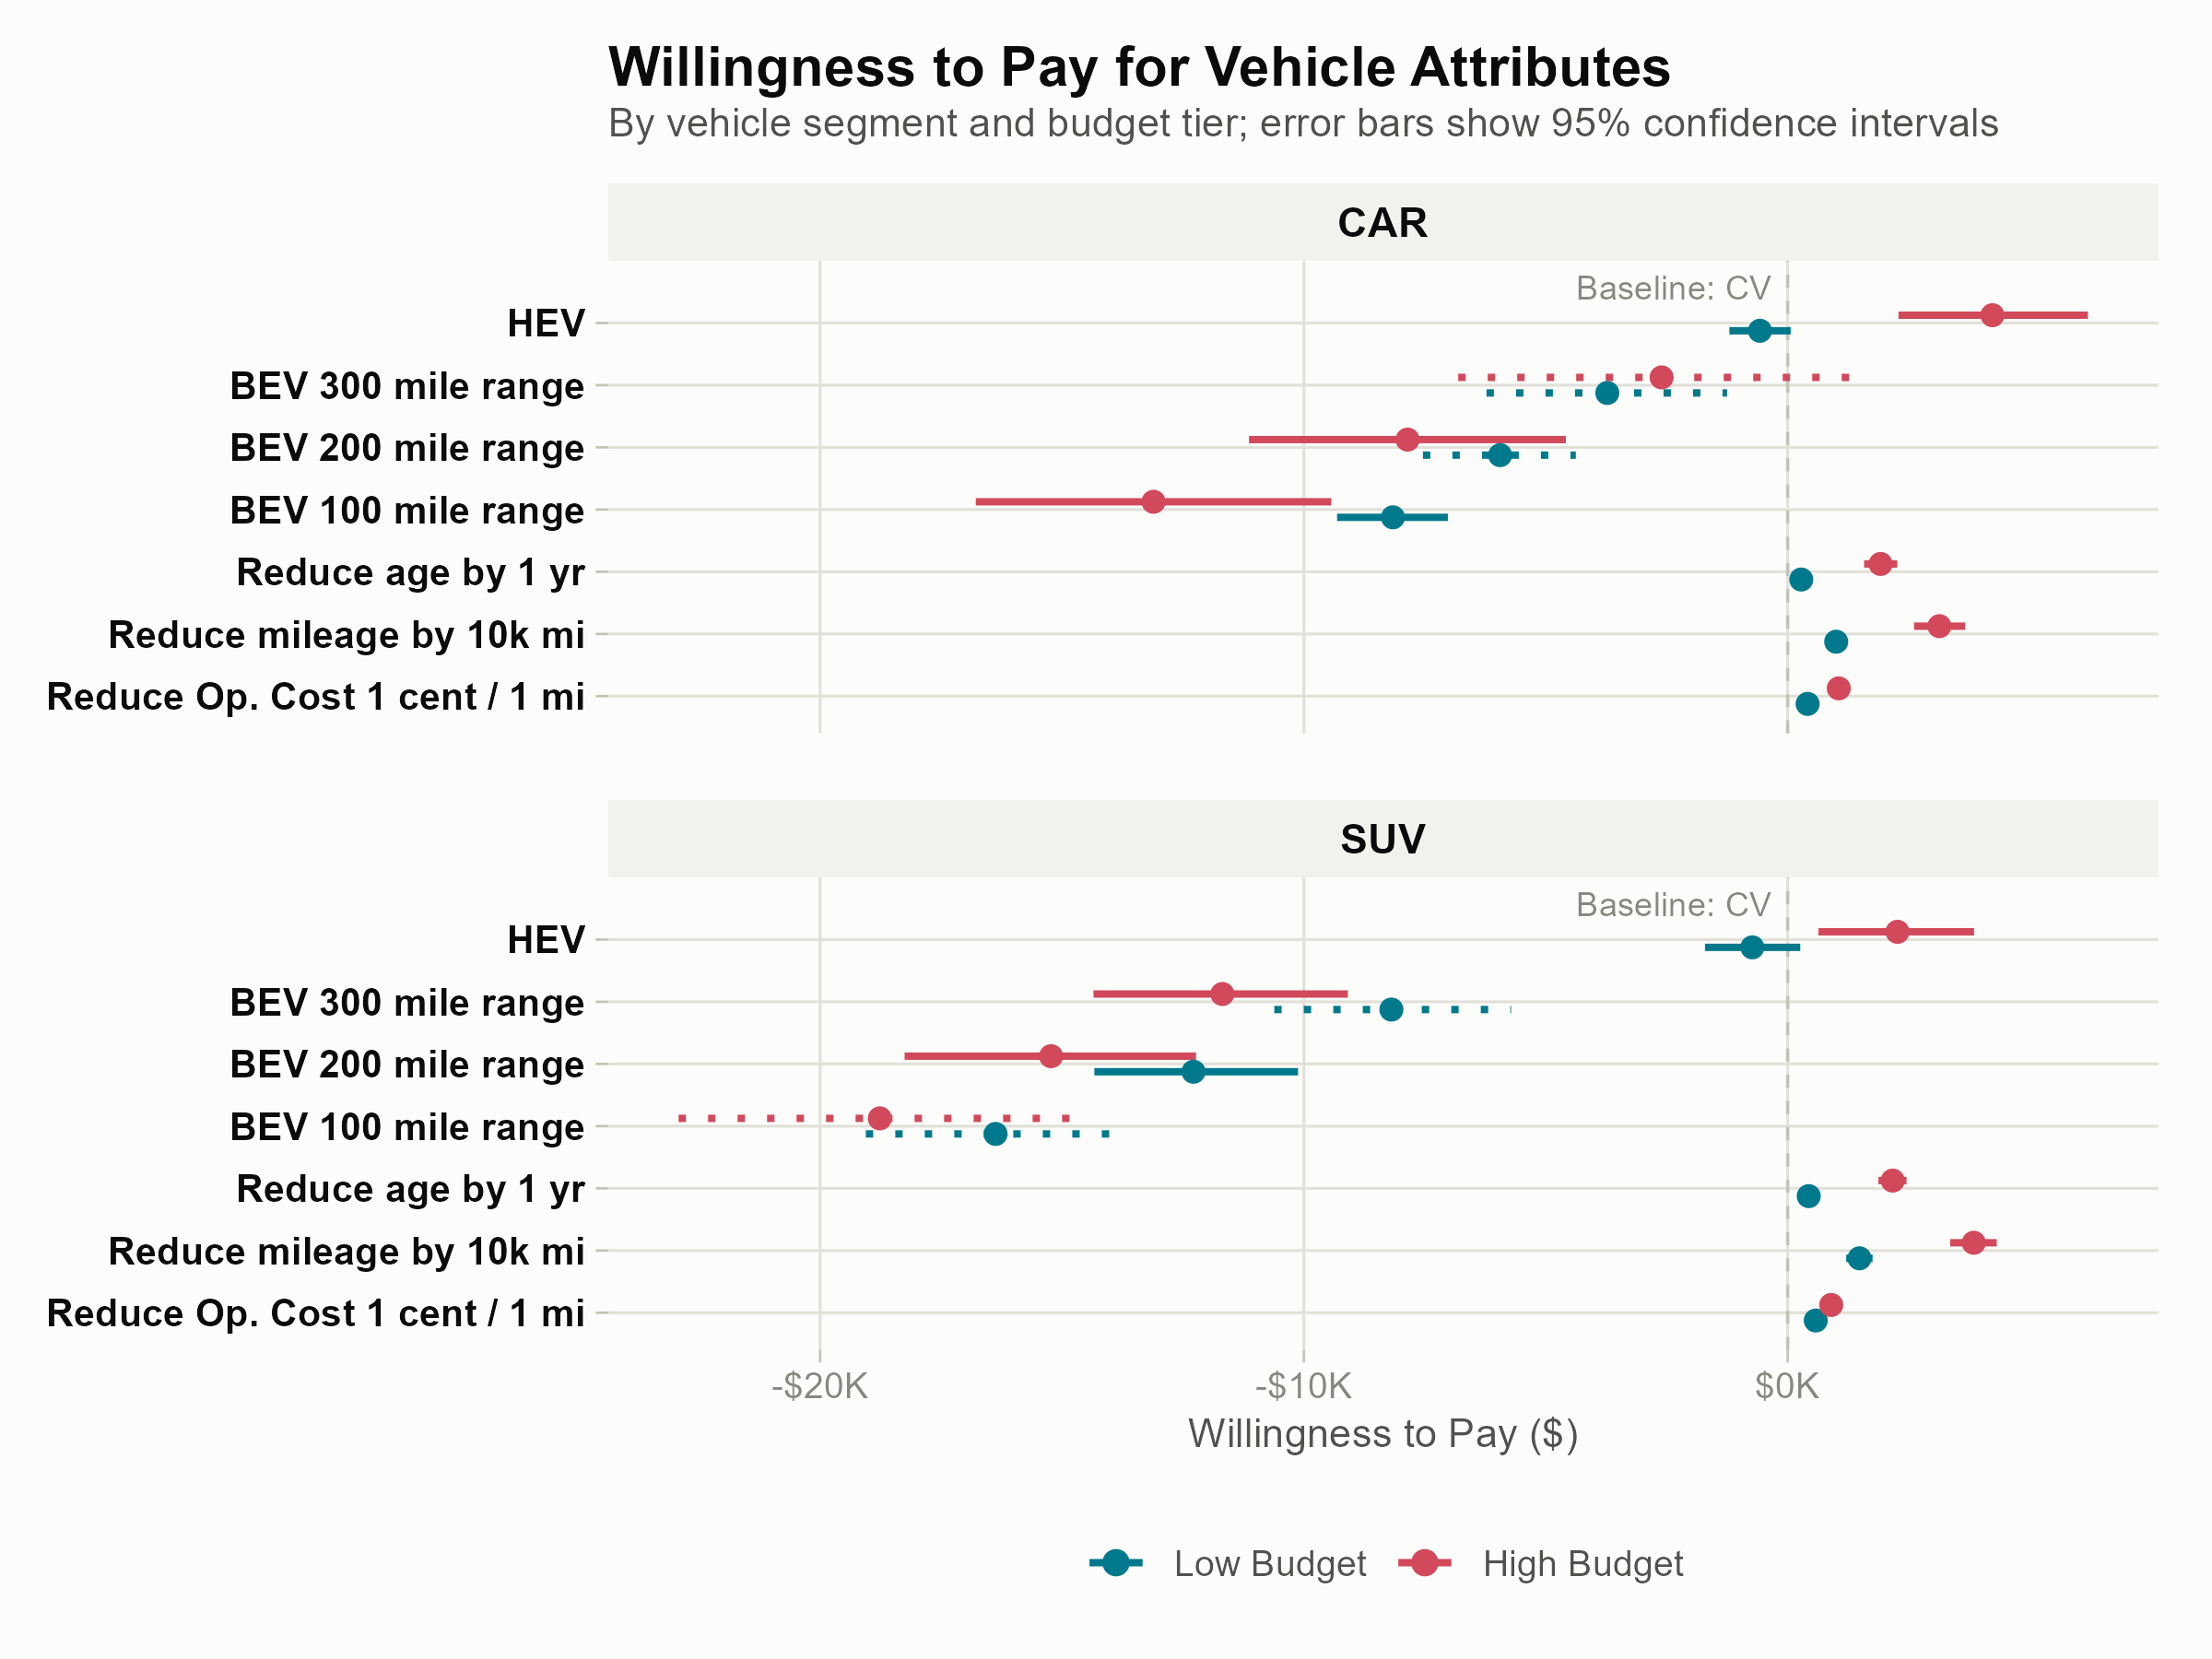
\includegraphics[width=\linewidth, height=0.85\textheight, keepaspectratio]{../../code/output/images/vehicle_analysis/wtp_plot_vehicle_attributes.png}
    \caption{Willingness to pay for vehicle attributes, by vehicle segment and budget tier (95\% confidence intervals shown; values in thousands of dollars). For the BEV range configurations, solid intervals mark WTP calculated within the range shown to that segment and dotted intervals mark WTP extrapolated beyond it.}
    \label{fig:vehicle_wtp}
\end{figure}

\clearpage
\begin{center}
{\fontsize{14}{17}\selectfont\textbf{Consumer Valuation of Battery Health Attributes in Used Battery Electric Vehicle Markets: A Discrete Choice Experiment}\par}
\vspace{0.5em}
{\fontsize{10}{12}\selectfont
Xiatian Iogansen\textsuperscript{1,2},
Zain Hoda\textsuperscript{1},
Christina Gore\textsuperscript{2},
Joshua D. Kneifel\textsuperscript{2},
Sindhu Ranganath\textsuperscript{1,2},
John P. Helveston\textsuperscript{1}\par}
\vspace{0.3em}
{\fontsize{10}{12}\selectfont
\textsuperscript{1}Department of Engineering Management and Systems Engineering, George Washington University\par
\textsuperscript{2}Applied Economics Office, Engineering Laboratory, National Institute of Standards and Technology\par}
\end{center}
\vspace{-1.5em}

\section*{Background}

Used vehicle transactions account for roughly 70\% of U.S. passenger vehicle purchases \parencite{bts2023}, and used BEVs are entering the secondary market at an accelerating pace \parencite{coxautomotiveinc.EVMarketMonitor2025}. Despite this, 52\% of U.S. adults are unlikely to consider a used BEV purchase \parencite{fernandesUSUnderstandingConsumer2023}, primarily citing uncertainty about battery condition. This information gap suppresses demand and prevents efficient pricing in the secondary market.

\section*{Data and Method}

We administered an online discrete choice experiment (December 2025--April 2026) to 3,072 U.S. adults intending to purchase a used car or SUV within two years. Each respondent completed six choice tasks among three hypothetical used BEVs or a no-choice option, varying mileage, price, electric range at Year~3, annual battery degradation rate, and battery refurbishment history. The design was stratified by body type and budget, and half the sample received extended battery cost and warranty information. We estimate a six-class Latent Class Choice Model on 2,916 respondents with complete covariate data (17,496 choice observations); class-specific WTP is the negative ratio of the attribute coefficient to the price coefficient.

\section*{Results}

The six classes differ markedly in battery quality sensitivity, price responsiveness, and market engagement; the attached figure (Figure~\ref{fig:lc6_class_profiles}) shows more details on each class.

\textbf{Class 1: Battery Health Attentives (22.7\%).} Highest range loss aversion (about \$2,300 per percentage point) and clear refurbishment penalties.

\textbf{Class 2: Multi-Attribute Maximizers (20.8\%).} Highest premium for a minimum viable range (\$11,830) and large refurbishment penalties (about -\$6,000).

\textbf{Class 3: Range-Focused, EV-Knowledgeable (16.6\%).} Very high WTP for range below 130 miles (\$38,700 per 100 miles); negligible refurbishment penalties.

\textbf{Class 4: Budget-Constrained, Low-WTP (12.8\%).} Largest price sensitivity and modest WTP for any attribute, yet 91.2\% never opt out.

\textbf{Class 5: Opt-Out Dominant, BEV-Skeptical (8.7\%).} 75.4\% chose no vehicle in all six tasks; most WTPs are indistinguishable from zero.

\textbf{Class 6: Low-Engagement (18.5\%).} Near-zero price coefficient, consistent with attribute non-attendance; WTP estimates treated as unreliable.

Classes~1 and~2 (43.5\%) prioritize battery health and are the primary market for standardized battery health certification.

\begingroup
\setlength{\bibitemsep}{0pt}
\setlength{\bibnamesep}{0pt}
\renewcommand{\bibfont}{\scriptsize}
\printbibliography[heading=none]
\endgroup

\clearpage
\begin{landscape}
\begin{figure}[H]
    \centering
    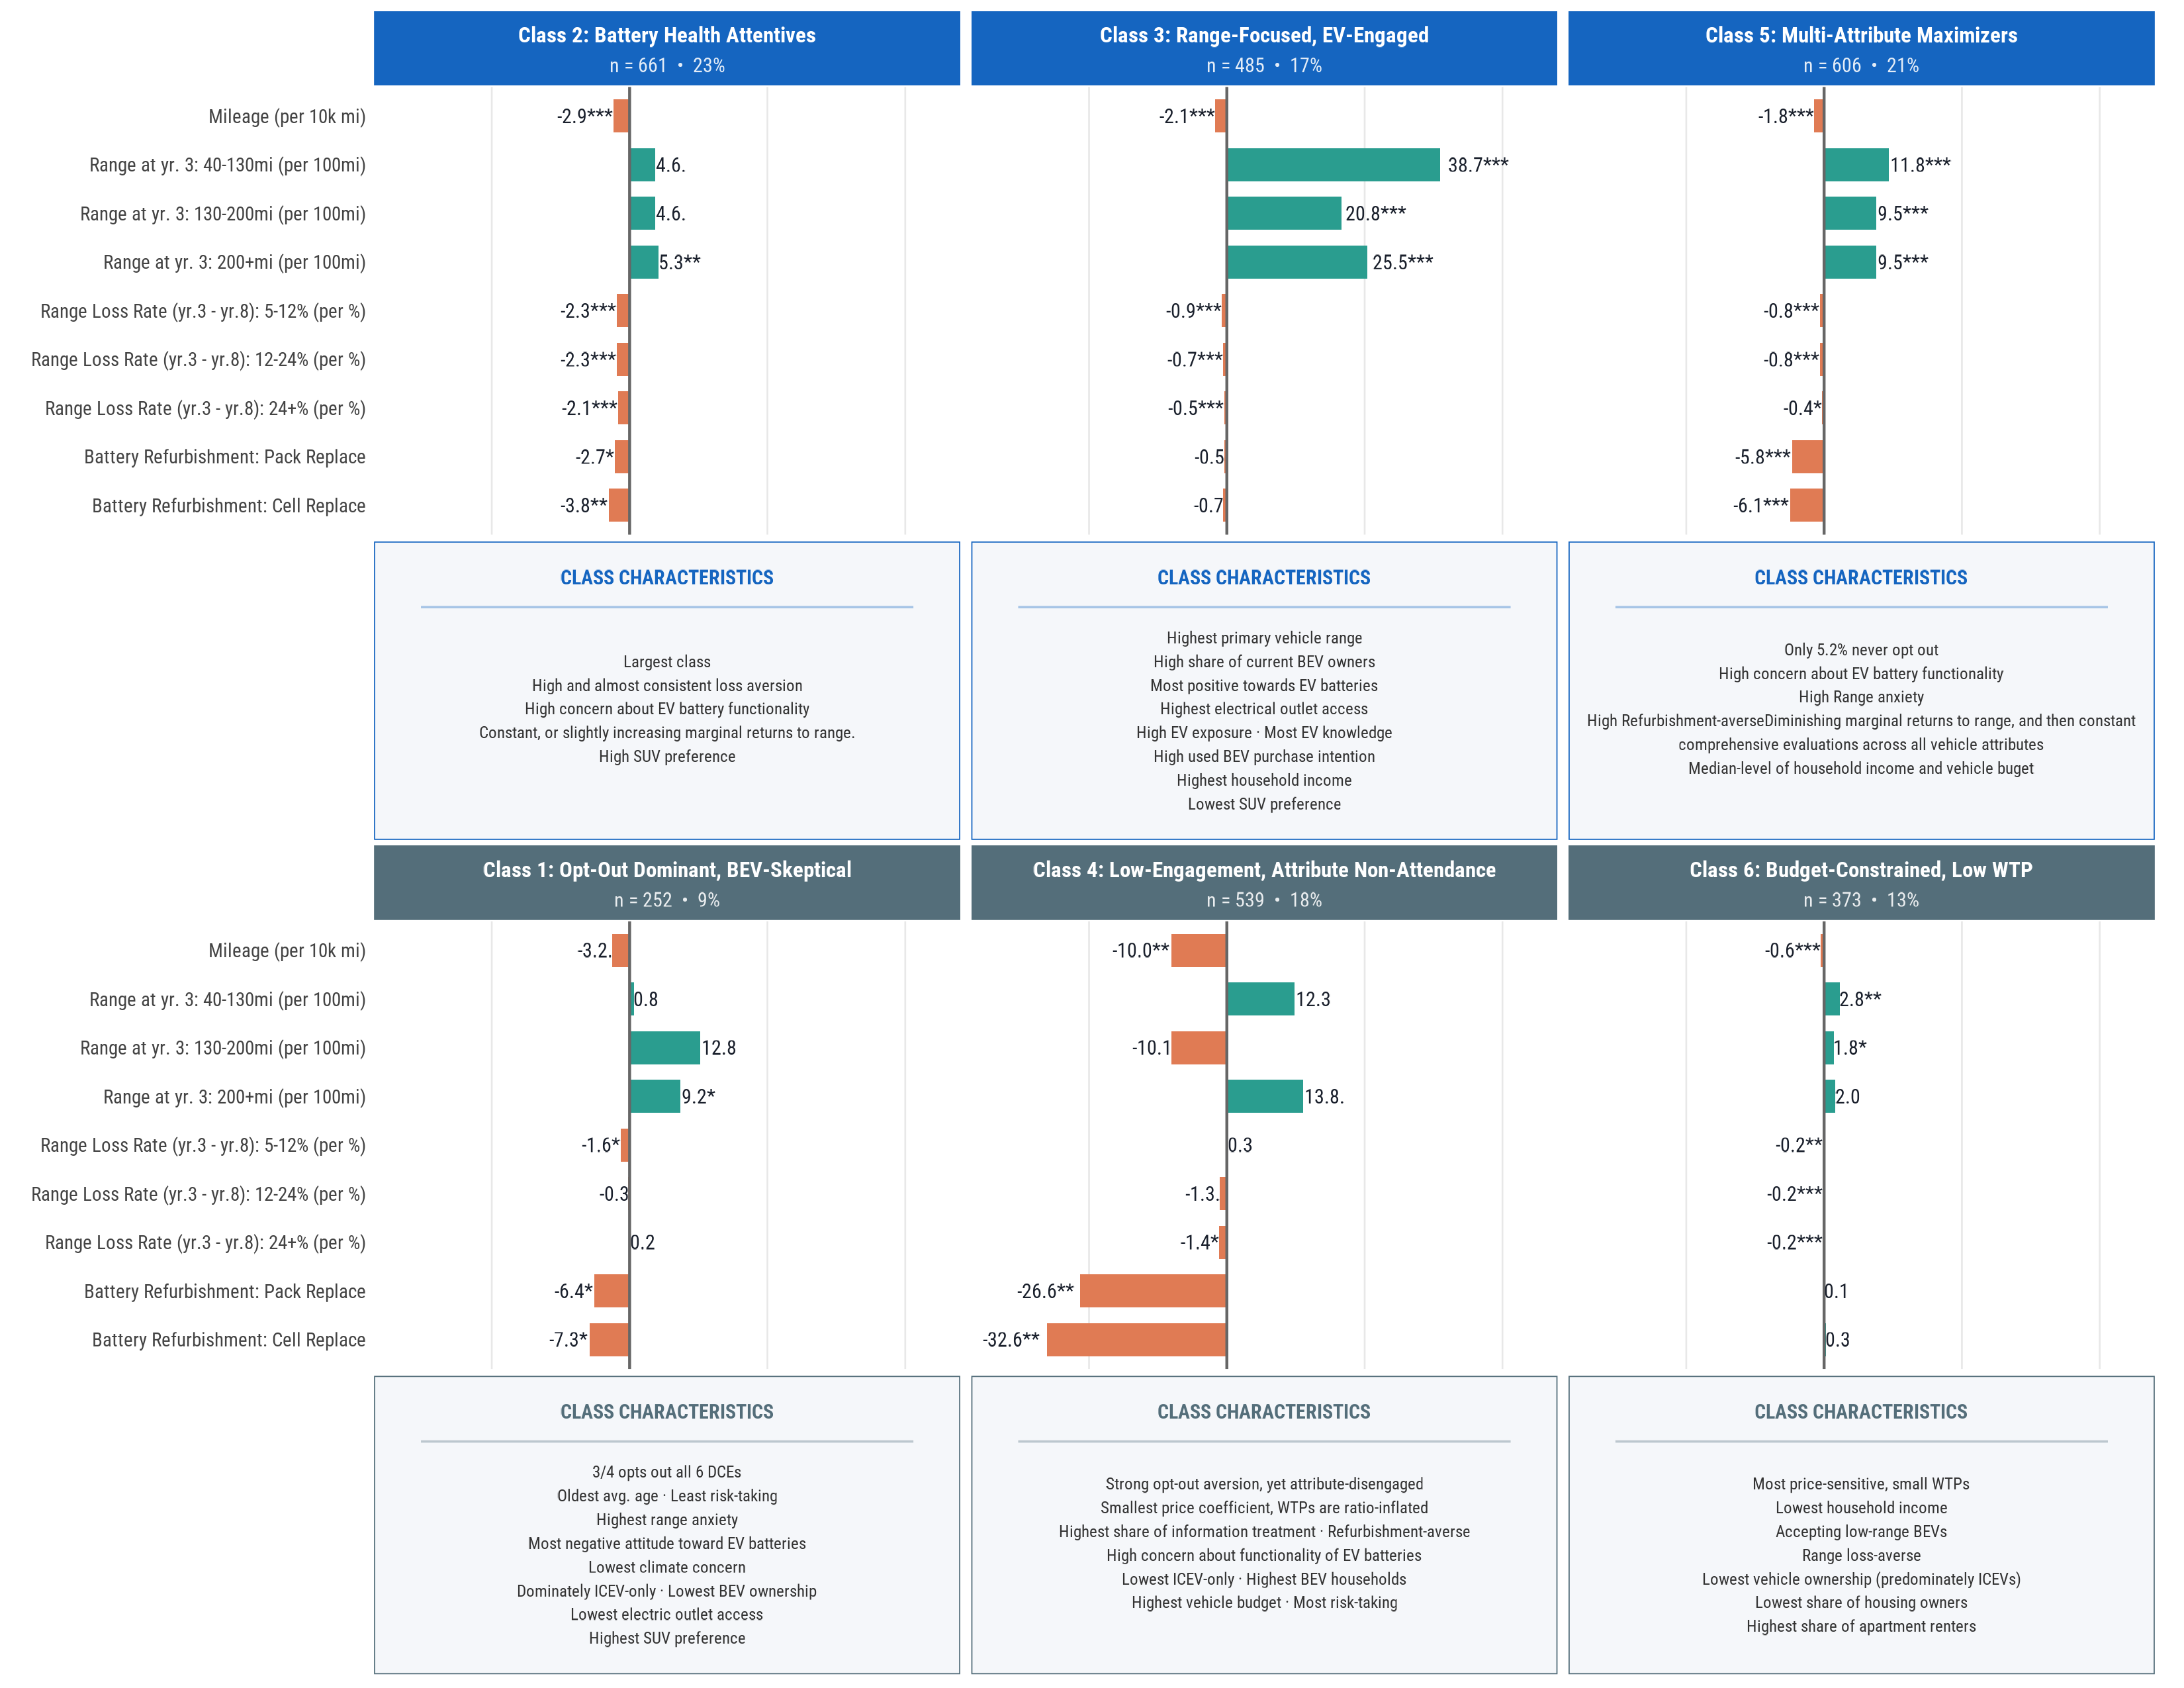
\includegraphics[width=0.94\linewidth, keepaspectratio]{../../code/output/model_output/battery_analysis/apollo/0_lc6_class_profiles_no_optout.png}
    \caption{WTP and class profile summary.}
    \label{fig:lc6_class_profiles}
\end{figure}
\end{landscape}

\end{document}
